\documentclass[11pt, a4paper, leqno]{article}
\usepackage{a4wide}
\usepackage[T1]{fontenc}
\usepackage[utf8]{inputenc}
\usepackage{float, afterpage, rotating, graphicx}
\usepackage{epstopdf}
\usepackage{longtable, booktabs, tabularx}
\usepackage{fancyvrb, moreverb, relsize}
\usepackage{eurosym, calc}
% \usepackage{chngcntr}
\usepackage{amsmath, amssymb, amsfonts, amsthm, bm}
\usepackage{caption}
\usepackage{mdwlist}
\usepackage{xfrac}
\usepackage{setspace}
\usepackage[dvipsnames]{xcolor}
\usepackage{subcaption}
\usepackage{minibox}
\usepackage{verbatim}
% \usepackage{pdf14} % Enable for Manuscriptcentral -- can't handle pdf 1.5
% \usepackage{endfloat} % Enable to move tables / figures to the end. Useful for some
% submissions.

\usepackage[
    natbib=true,
    bibencoding=inputenc,
    bibstyle=authoryear-ibid,
    citestyle=authoryear-comp,
    maxcitenames=3,
    maxbibnames=10,
    useprefix=false,
    sortcites=true,
    backend=biber
]{biblatex}
\AtBeginDocument{\toggletrue{blx@useprefix}}
\AtBeginBibliography{\togglefalse{blx@useprefix}}
\setlength{\bibitemsep}{1.5ex}
\addbibresource{refs.bib}

\usepackage[unicode=true]{hyperref}
\hypersetup{
    colorlinks=true,
    linkcolor=black,
    anchorcolor=black,
    citecolor=NavyBlue,
    filecolor=black,
    menucolor=black,
    runcolor=black,
    urlcolor=NavyBlue
}


\widowpenalty=10000
\clubpenalty=10000

\setlength{\parskip}{1ex}
\setlength{\parindent}{0ex}
\setstretch{1.5}


\begin{document}

\title{Revision of: Forecasting economic activity using a text-classification model\thanks{Fabian Schmidt, University of Bonn. Email: \href{mailto:schmidt.fabian-christian@t-online.de}{\nolinkurl{schmidt [dot] fabian-christian [at] t-online [dot] de}}.}}

\author{Fabian Schmidt}

\date{
    \today
}

\maketitle


\begin{abstract}
    With this project, I am trying to improve forecasts of economic activity in the short-run by adding a measure of sentiment to the analysis. To do so, I first webscrape a thousand headlines from the German newspaper website "welt.de" and then analyze them using a text-classification model.
    I then hand-label a few of the headlines and train the model. I then use this model to again analyze the headlines and compare the results. Lastly, the sentiment labels are used in a VAR model to forecast economic activity in the short-run.\\
    The results are as follows:
\end{abstract}

\clearpage


\section{Introduction} % (fold)
\label{sec:introduction}

With this project, I am trying to improve forecasts of economic activity in the short-run using a text-classification or more specifically sentiment analysis model using newspaper headlines. The goal of this project is to see if a text-classification model can improve forecasts from standard econometric models (e.g. autoregressive models) in the short-run by adding a measure of sentiment to the analysis.
A secondary goal is to analyze how much data is needed, what kind of data is most useful and which model one should pick, and how much tuning needs to be done to forecast short-run economic activity using newspaper headlines.
This template is using the econ-project-template \citet{Gaudecker2023}.
The rest of the paper is structured like the following:
\begin{enumerate}
    \item The idea behind the project will be swiftly explained and similar research that influenced the choice of the project will be mentioned and briefly summarized.
    \item The setup of the project will be documented. Datasets and the issue with getting this data will be discussed. The used model and methods to analyze the sentiment of the headlines will be presented.
    \item The results of this project will be presented and discussed.
    \item Extensions and improvements of the project will be discussed.
\end{enumerate}

% section introduction (end)
\section{The idea behind the project}
In this section, I will discuss the idea behind this project as well as mention a couple of similar research projects that were influential in my choice of this project. This section has by no means the ambition to provide a complete overview of all the literature similar to this project, but is rather a history of thought behind the project.

The idea behind this project is to see if text-classification machine learning models can improve forecasting of economic relevant variables. Such an improvement is desirable since an improvement in forecasts can lead to better information availability and, therefore, improve decision-making by firms, households, institutions, and governments. The traditional approach to forecasting macroeconomic variables usually features auto-regressive models that try to put traditional economic variables like inflation or the unemployment rate into relation to each other as well as into relation to each other's lags and exogenous shocks. Alternatively, dynamic stochastic general equilibrium (DSGE) models are used to forecast macroeconomic variables by capturing the intricate interplay of economic agents in different market environments, enabling a more comprehensive understanding of how various factors influence the trajectory of key economic indicators. Both of these approaches, however, can struggle to make precise short-term forecasts for macroeconomic variables. For example, during the start of the COVID-19 crisis forecasting models were not able to correctly identify the magnitude of the exogenous shock hitting the economy resulting in the ECB having to re-evaluate their forecasting models \parencite{Battistini2021}. Furthermore, in the aftermath of the COVID-19 pandemic forecasting models were, again, unable to correctly predict the rise in inflation and the duration of how long inflation would stay at this high level. One possible explanation for why this might be the case is that expectations of the general public influence the short-term behaviour of these variables in ways that are challenging to capture for these models.
In recent history, machine learning models were introduced to forecasting with the idea that large deep learning models might be able to infer insights from the data that standard auto-regressive models could not find. One strand of the literature also looked at designing more subjective measurements and using these for forecasting economically relevant variables. For example, \textcite{Denes2022} used Twitter data to measure inflation perception using a random forest. They show that their indicator is consistent with measured inflation perception by household surveys. They also show that their indicator is strongly correlated with the actual inflation rate which could spark the idea that such a model could be used for forecasting inflation.

Another study is taking a similar approach. The Finance and Economics Discussion Series (FEDS) working paper by \textcite{Adams_2023} uses the FinBert model to analyze the sentiment of Twitter data to then use this sentiment indicator to predict next-day stock market returns.

My approach is building on this literature. However, rather than focusing on a specific group like Twitter users, I try to find an approach that resembles the sentiment of the overall population. Additionally, I do not focus on the financial market, but rather on real economic activity.

Potential research questions for this project, thus, are: Can text-classification machine learning models improve forecasts for real economic activity? Are newspaper articles or headlines a good indicator of current political, economic, and financial developments and the sentiment related to those developments? Which models can be used to do sentiment analysis? How much data is needed to train such a model?
I will try to answer some of these questions in this project. These questions can then be, potentially, further investigated in follow-up work like, for example, a master's thesis.

\section{The Setup of this Project}

To do this project, I need two sources of data. One indicator for economic activity and one source of data that is representative of the public sentiment about current political, economic, and financial developments inside of the economy. I decided to focus on one specific country since trying to analyze the sentiment of the entire world using text-classification models is most likely not possible and most definitely too big of a task for this project. Since I am from Germany and I am doing this project at a German university, I decided to focus on the German economy and the German population.

As a source of data to analyze public sentiment, I chose to use newspaper headlines. That is because, firstly, a lot of German citizens tend to read classical newspapers. A survey done by the *Zeitungsmarktforschung Gesellschaft (ZMG)* in 2022 on behalf of the German Association of Digital Publishers and Newspaper Publishers (BDZV) found that about 80 percent of the German population above 14 years old read newspapers either physically or online regularly. As a consequence, it could be expected that newspapers could potentially influence the sentiment of the general public on current developments and, secondly, it could be expected that journalists and newspaper agencies have a good understanding of the overall public sentiment of the population that is reflected in their articles as well. Therefore, I decided to choose newspaper headlines as an indicator of overall public sentiment.

I focused on headlines rather than whole newspaper articles since, firstly, usually the headline of an article is sufficient to analyze the overall sentiment of the article. Secondly, whole newspaper articles are usually not open-accessible without paying for access or receiving access through an institution which was not possible in my case. Furthermore, analyzing whole newspaper articles would most likely make the process that is used for sentiment analysis done by machine learning models more difficult since more inputs per headline would most likely also require more data to tune the model with. Additionally, this amount of data could be difficult for soft- and hardware to deal with. This would have been most definitely the case for the soft- and hardware that I was working with. Therefore, I decided to focus on headlines rather than on whole newspaper articles.

Since newspaper headlines are not openly accessible in a public database, but rather can be found on the websites of newspapers, I decided to webscrape them from the website of the newspaper. I chose the newspaper "Die Welt" as the representative newspaper for Germany since the newspaper is one of the biggest daily newspapers in Germany and it has all of their past headlines openly accessible on their websites making it much easier to webscrape them. An additional benefit from choosing "Die Welt"'s website to webscrape the data from is that they have categorized their newspaper articles into easily distinguishable categories. Therefore, it was easy for me to only choose newspaper headlines that were located in the right category so that I would not analyze headlines that are not reflective of the general public's current sentiment. The code for the webscraping can be found in the source code of my GitHub repository.

As the second source of data, I needed an indicator of economic activity in Germany. As criteria for choosing this indicator, I tried to find an indicator that was available daily and was representative of real economic activity in Germany. The latter I chose as criteria because I try to analyze the overall public sentiment of the population in Germany. Therefore, only focusing on specific markets would not be coherent with the overall idea of forecasting overall economic activity with sentiment analysis.
I chose to use the daily truck toll mileage indicator issued by the German *Bundesbank* and the German *Federal Statistical Office*. This indicator is a relatively new indicator for economic activity and, therefore, parts of it are still experimental. The index is supposed to provide approximate indications of the development of industrial production in Germany at an early stage. The index developed by the Federal Office for Goods Transport traces the development of the mileage of large trucks (with four or more axles) on German motorways. It is calculated from digital process data of the truck toll collection system. The daily data of the truck toll mileage index are also published in calendar and seasonally adjusted form; the adjustment is carried out by the German Bundesbank. As the methods of seasonal adjustment of daily data are still under development, the seasonally adjusted daily data of the truck toll mileage index are described as experimental (German Federal Statistical Office website- Destatis).

I chose this specific indicator since it is available daily and it provides a new source for measuring economic activity in Germany that has not been used a lot, yet.

Before using this indicator, I had to detrend the indicator since the focus of my analysis was on analyzing if newspaper headlines can help to better detect short-term developments. Therefore, I wanted to remove the long-run trend from the data. I did so by applying the Hodrick-Prescott filter. The Hodrick-Prescott filter is a statistical filter specifically developed for finding the trend and cycle component of macroeconomic variables from the data. As a consequence, the filter was perfectly suited for my specific task.

The other components that I needed for my project were a sentiment analysis model for analyzing newspaper headlines and multiple forecasting models for analyzing if the analyzed sentiments could improve forecasting performance. Since I needed an ender-only model for analyzing sentiments, a Bert model was an obvious choice. I decided to use the multilingual-sentiment-newspaper-headlines model by Zachary Dickson which is accessible via huggingface. This model is a fine-tuned version of the bert-base-multilingual-cased model that was fine-tuned on a dataset of 30 thousand newspaper headlines in German, Polish, English, Dutch, and Spanish. The dataset contains six thousand headlines in each of the five languages.
One benefit in choosing this specific model is that this model was already partly trained on newspaper headlines from the newspaper "Die Welt" as documented on the model's webpage.

The other model components that I needed were multiple forecasting models for forecasting economic activity in Germany partly using the previously created sentiment indicator. For forecasting, I chose two more traditional models. The two traditional forecasting models that I chose were an ARMA model as a baseline model and a VAR model as the model using the sentiment indicator previously created.

\section{Results}

In the next section, I will present the results of the project. The results of the project can be summarized like the following: Using newspaper-analyzed sentiment labels did not improve forecasting economic activity as a whole. There is some indication that forecasting economic activity might improve in the very short-run (1-4 days) using sentiment labels. The main issue with using sentiment labels for forecasting economic activity seems to be that to forecast multiple periods into the future one also has to forecast the sentiment labels themselves into the future which I did not manage to do very precisely. Therefore, forecasting accuracy seems to get drastically more imprecise after a couple of days. Additional issues with the sentiment indicator were that while the sentiment analysis of single headlines was relatively precise and I was even able to improve the performance slightly by fine-tuning the model on a small hand-labelled dataset, the model was not able to analyze the sentiment of all headlines on one specific day. This was the case due to a limitation of input embeddings in the configuration of the model. However, even when using a smaller set of headlines and trying to analyze them all together at once, the model still did relatively poorly at analyzing the sentiment of these headlines. As a consequence, I had to analyze each headline separately and then took the mean over all the sentiment labels of that day. This led to the sentiment labels being rather imprecise when being compared to a small hand-labelled dataset due to there not being any weighting for all the headlines of a specific day. Possible improvements to the labelling process and how that could affect the forecasting results will also be discussed here.

I will now present some of the results of the project in detail and finish this section by discussing possible improvements and extensions.

Firstly, I will analyze the results of the sentiment labelling of the newspaper headlines. To do so I will first analyze the classification report of the test data for the zero-shot classification model and then do the same for the fine-tuned model. I will then compare their results and talk about the implications of these results. As the dataset for the evaluation, I used 300 hand-labelled headlines that I labelled myself. While I tried to remove personal biases and opinions when labelling the dataset my opinion and the sentiment that I sort to certain headlines is, of course, also just subjective and the scores that I will present here should be viewed under this consideration.

\input{../tables/classification_report_zero_shot_classification_model.tex}



\input{../tables/confusion_matrix_zero_shot_classification_model.tex}

Above, one can see the classification report and confusion matrix of the zero-shot classification done by the sentiment analysis model. As we can see the macro and weighted precision of the zero-shot classification is better than the recall score of these two. Just the recall accuracy of the label "negative" exceeds the precision accuracy. From the confusion matrix, one can infer that headlines that were "neutral" labelled were often classified as "negative" leading to the low precision score for the "negative" label. Furthermore, we can observe that headlines that were labelled "positive" by myself were labelled as "negative" by the model with the same probability as being labelled with their "true" label. Therefore, one can conclude that the model that was not fine-tuned seems to struggle the most with identifying newspaper headlines that were classified as "positive" by myself.

At next, I will discuss the results of the fine-tuned version of the model. As the dataset for the fine-tuning I, again, used the 300 hand-labelled headlines. 200 of those were randomly selected as training data while 50 were selected as evaluation and 50 as test data. The metric that I used was the macro f1-score. I decided to use the macro f1-score rather than the weighted f1-score since my data is slightly imbalanced. I decided to go for the f1-score since I could not find any reason why one would prefer the precision or the recall score in my specific scenario.
I decided to only use one training epoch for my model since when I experimented with different amounts of training epochs I found that the model was overfitting the data after one training epoch almost every time. Therefore, I only chose one.

\input{../tables/classification_report_finetuned_model.tex}



\input{../tables/confusion_matrix_finetuned_model.tex}

Above, we can see the classification report and confusion matrix of the fine-tuned model. As one is able to recognize almost all scores have improved due to fine-tuning. Especially the precision score of the model has improved significantly while the recall score has only improved slightly. The only slight improvement in the recall score is mostly due to a significantly worse recall score for the label "negative". The recall score still improved since, at the same time, the recall score for the label "neutral" improved even more than the recall score for the label "negative" got worse.
Looking at the confusion matrix, we can identify that all of the "negative" labelled headlines that were incorrectly identified were identified as "neutral". Furthermore, also for the fine-tuned model the probability of a "positive" labelled headline being labelled as "positive" by the model was as high as the probability of being labelled "negative". So it still seems that the model struggles the most with headlines that were identified as "positive" headlines.

I also tested the performance of both models on the test dataset. I will not list the results here since they are very similar to the results discussed above and, as a consequence, would not provide any new insights.

Lastly, I also tested both models on a small dataset that was also hand-labelled by myself. However, rather than labelling individual headlines I labelled all headlines of a specific day giving them one overall label for one day. I then let both models label the entire dataset and took the mean of all labels of all the headlines from one day as the overall sentiment of that specific day.
The mean squared error for the zero-shot classification model compared to the my labels was equal to while the mean squared error for the fine-tuned model was equal to. When comparing the mean squared error for both models, the fine-tuned model has a lower error compared to the zero-shot classification thereby indicating that fine-tuning does not only improve the performance of the model in classifying individual headlines, but the improvement in classifying individuals also results in a more accurate sentiment score for the entire day. This score most likely would greatly improve for both models if there was some kind of weighting attached to each individual headline of a specific day, but that is an improvement that I will discuss later.
I chose to use the mean squared error as a metric rather than the classification report or the confusion matrix since I intentionally decided not to round the scores for the daily sentiment to fit one specific label since I believe that it is a good thing that the daily sentiment score is rather a spectrum in between the three possible labels rather than always having to be one specific label of the three.

At next, I will discuss the results of the forecasting part of this project.

For forecasting economic activity I decided to use two traditional time-series forecasting models, an ARMA model and a VAR model. I used the ARMA model as a baseline model while the VAR model featured the newly created sentiment variable and where, therefore, compared to the baseline model.

\input{../tables/summary_statistics_ARIMA_model.tex}



\VerbatimInput{../tables/summary_statistics_VAR_model.txt}



\begin{figure}[h!]
    \includegraphics[width=\textwidth]{../figures/ARIMA_forecasts_cycle.png}
\end{figure}
\newpage
\begin{figure}[h!]
    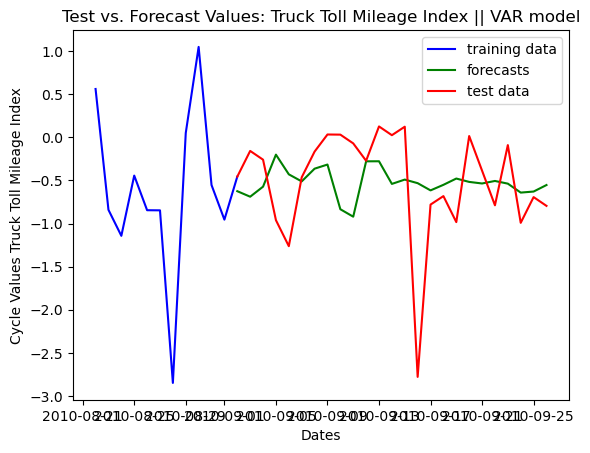
\includegraphics[width=\textwidth]{../figures/VAR_forecasts_cycle.png}
\end{figure}




\section{Discussion}

Lastly, I will talk about possible improvements for this project.
The main improvements that I would have made next if there was more time available would have been to improve the accuracy of the daily sentiment label. To do so I would have created more data to fine-tune the model with and also created a deep learning model that would calculate a weight for each headline of a specific day. This could improve the accuracy of the model immensely and thereby could also improve the forecasting performance of the VAR model since the process of fine-tuning with just a small dataset as I did in this project improved the forecasts of the VAR model as well. To create such a deep learning model I would have labeled a dataset of headlines based on their perceived importance for the German economy and then trained the model on that dataset. One could have then used the label from this model together with the score that the sentiment analysis model provided when analyzing the headlines, lowering the weight of headlines with a low score and increasing the weight of headlines with a high score, to weight each individual headline of that specific day. Those two improvements would hopefully improve the performance of the daily sentiment label immensely and could lead to an improvement in forecasting as well.
The second major improvement that I would have done is to improve the forecasts for the sentiment label values. To do so one would have to experiment with different approaches and even more additional variables to see if the sentiment label values can be forecasted more precisely.
Two last possible improvements for this project would have been to, firstly, use a different time horizon to examine and, secondly, to use other sources of data. The time horizon that I chose to examine was chosen arbitrarily and, therefore, I did not do further investigations if specific time horizons would have led to other conclusions. Such examinations, however, could have been valuable.
The same could be said about using other sources of data. Using different representative sources for public sentiment as well as different indicators and indexes for economic activity could, again, highlight valuable insights. Nevertheless, due to the time restriction of this project, I was not able to extend my investigations in these directions and those investigations will have to follow in future work.


\setstretch{1}
\printbibliography
\setstretch{1.5}


% \appendix

% The chngctr package is needed for the following lines.
% \counterwithin{table}{section}
% \counterwithin{figure}{section}

\end{document}
